\documentclass[12pt,a4paper]{article}
\usepackage[a4paper, left=2.5cm,right=2.5cm,top=3cm,bottom=3cm]{geometry}
\usepackage[utf8]{inputenc}
\usepackage[spanish]{babel}
\addto\captionsspanish{
	\renewcommand\chaptername{}
	\renewcommand\appendixname{Anexo}
	\renewcommand\appendixpagename{Anexos}
	\def\tablename{Tabla}
	\def\listtablename{\'Indice de tablas}
}
\usepackage{ucs}
\usepackage{subfig}
\usepackage{float}
\usepackage{amsmath}
\usepackage{amsfonts}
\usepackage{amssymb}
\usepackage{graphicx}
\usepackage{listings}
\usepackage{color}
\usepackage[T1]{fontenc}
\usepackage[scaled]{beramono}
\usepackage{upquote}
\usepackage{xcolor}
\usepackage{listings}
\usepackage{caption}
\usepackage{chngcntr}
\usepackage{endnotes}
\usepackage{float}
\usepackage{hyperref}
\usepackage{wrapfig}
\usepackage{fancyhdr}
\usepackage{emptypage}
\usepackage{times}
\usepackage{array}
\usepackage{setspace}
\usepackage{multirow}
%\usepackage{subfigure}
\usepackage{verbatim}
%\usepackage{tabulary}
%\usepackage{graphicx,subfigure}
\usepackage[bottom]{footmisc} 
\usepackage{appendix}
\usepackage{mathtools}
\usepackage{textcomp}


%listing, code style
% Define a custom color
\definecolor{backcolour}{rgb}{0.95,0.95,0.92}
\definecolor{codegreen}{rgb}{0,0.6,0}

% Define listing style
\lstset{
	language=python,
	tabsize=4,
	rulecolor=,
	basicstyle=\scriptsize,
	upquote=true,
	aboveskip={1.2\baselineskip},
	columns=fixed,
	numbers=left,
	showstringspaces=false,
	extendedchars=true,
	breaklines=true,
	prebreak = \raisebox{0ex}[0ex][0ex]{\ensuremath{\hookleftarrow}},
	showtabs=false,
	showspaces=false,
	showstringspaces=false,
	identifierstyle=\ttfamily,
	keywordstyle=\color[rgb]{0,0,1},
	commentstyle=\color[rgb]{0.133,0.545,0.133},
	stringstyle=\color[rgb]{0.627,0.126,0.941},
} 


\renewcommand{\notesname}{Fuentes}
\renewcommand{\baselinestretch}{1.2}
\hypersetup{
	colorlinks,%
	citecolor=black,%
	filecolor=black,%
	linkcolor=black,%
	urlcolor=black
}

\begin{document}
	
\begin{titlepage}
	\centering
	%\null\vfill
	
\includegraphics[width=\textwidth]{FIGURES/Portada/Logo_portada.png} 
	\vspace{1.5cm}
	
	Universidad Politécnica de Madrid
	\\Escuela Técnica Superior de Ingeniería Aeronáutica y del Espacio
	\vspace{2cm}
	
	{\large MÁSTER UNIVERSITARIO EN SISTEMAS ESPACIALES}
	\vspace{2cm}
	
	{\LARGE MILESTONE 4}
	\vspace{1cm}
	
	{\large Ampliación de Matemáticas I}
	\vspace{4cm}
	
	\begin{center}
		\large{\textbf{\today}} \\
	\end{center}
	
	Autor: \\ Alberto García Rincón
	\vfill
\end{titlepage}

%****INDICES****
\newpage
\pagestyle{empty}
\tableofcontents	

%******DOC******	
\newpage
\pagenumbering{arabic}
\setcounter{page}{1}
\pagestyle{fancy} 

\section{Introducción}
En este trabajo se ha definido un nuevo problema, el oscilador armónico lineal, que se va a integrar mediante los distintos métodos de cálculo numérico que ya se han utilizado en trabajos anteriores y además se ha añadido un nuevo método de integración más: Leap Frog.

El oscilador armónico lineal queda definido por la siguiente ecuación diferencial:
\begin{equation} \label{osci}
	\ddot{x} + x = 0 
\end{equation}

Posteriormente se va a realizar el cálculo y análisis de las regiones de estabilidad de los distintos métodos de cálculo numérico utilizados hasta la fecha. 


\section{Código de Python}
\subsection{Diagrama de bloques}
\begin{figure}[H]
	\centering
	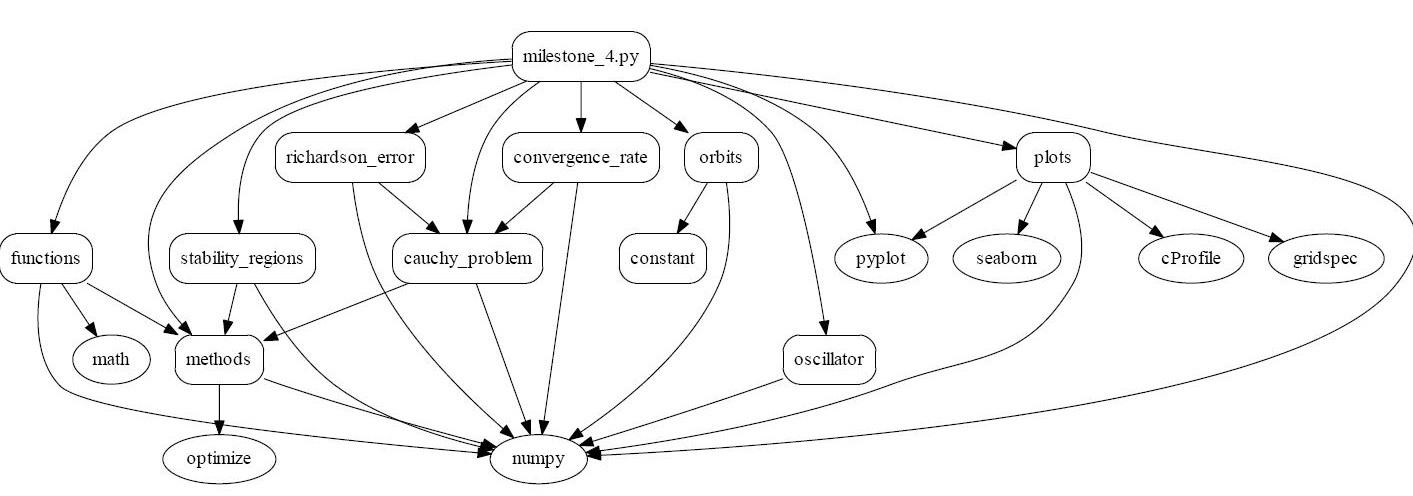
\includegraphics[width=0.99\textwidth]{FIGURES/mil4/codigo/diagram_milst4.JPG}
	\caption{Diagrama archivos Milestone 4.}
	\label{diagram}
\end{figure}

Para hacer funcionar este programa se debe ejecutar el programa principal denominado $milestone\_4.py$. Este programa se encarga de llamar al resto de funciones definidas en los respectivos archivos.

Se van a comentar los cambios introducidos respecto al trabajo de la semana pasada en el código de los archivos del programa.


\subsection{milestone\_4.py}
En el archivo principal se ha definido un nuevo problema a resolver, en este caso se trata del problema del oscilador armónico. Para ello se han definido unas condiciones iniciales de posición y velocidad, como se muestran en la figura \ref{main2}. También se ha definido un vector $Ut$ que contiene varios $\Delta t$, se realizarán simulaciones del problema del oscilador con estos incrementos de tiempo. 

El vector $mets$ contiene los distintos métodos de resolución que se van a utilizar para resolver el problema. 
\begin{figure}[H]
	\centering
	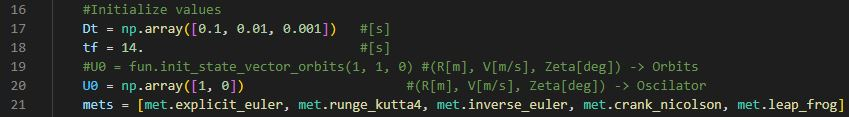
\includegraphics[width=0.9\textwidth]{FIGURES/mil4/codigo/main2.JPG}
	\caption{Iniciación de valores en el programa principal.}
	\label{main2}
\end{figure}

En la siguiente figura \ref{main3}, se muestra el código que permite la resolución del problema del oscilador armónico para los $\Delta t$ definidos en el vector anteriormente citado. De esto de encarga el primer bucle, siendo el segundo el que recorre el vector de los métodos definidos. Finalmente los valores de los resultados se almacenan en el vector de vectores $UU$, que ha sido inicializado anteriormente.  
\begin{figure}[H]
	\centering
	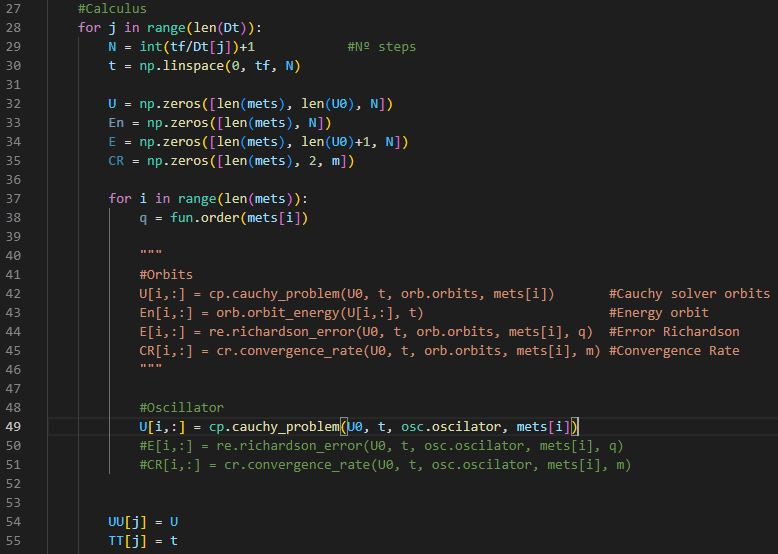
\includegraphics[width=0.9\textwidth]{FIGURES/mil4/codigo/main3.JPG}
	\caption{Código de cálculo de los valores del problema del oscilador armónico.}
	\label{main3}
\end{figure}

Unas líneas más abajo en el archivo principal. Se definen las condiciones para calcular las regiones de estabilidad de los diferentes métodos de cálculo y el bucle que recorre estos mismos. 

Desde este mismo bucle se llama a la función encargada de dibujar las distintas regiones de estabilidad. 
\begin{figure}[H]
	\centering
	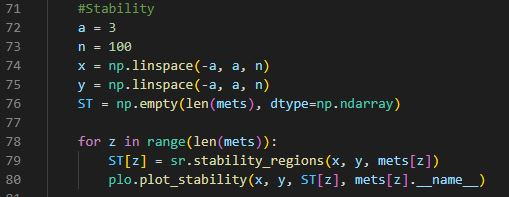
\includegraphics[width=0.75\textwidth]{FIGURES/mil4/codigo/main1.JPG}
	\caption{Código para cálculo de regiones de estabilidad.}
	\label{main1}
\end{figure}

\subsection{plot.py}
En este archivo se definen todas las funciones necesarias para dibujar las distintas gráficas de los resultados obtenidos.

La siguiente figura muestra el código de la función encargada de dibujar la posición y velocidad del oscilador para distintos $\Delta t$ calculados y para todos los métodos con los que se ha realizado el cálculo.

Se definen dos bucles: el primero para recorrer los métodos de cálculo y el segundo para recorrer los distintos $\Delta t$. Esta función permite que siendo llamada una única vez desde el programa principal, dibuje todas las gráficas de una vez.
\begin{figure}[H]
	\centering
	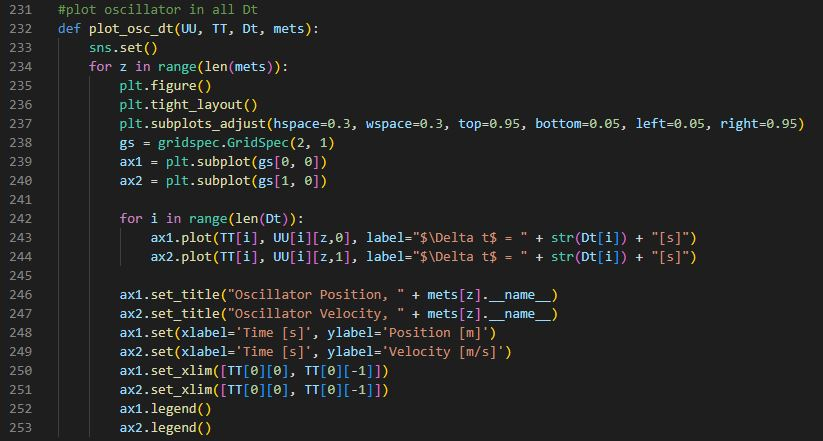
\includegraphics[width=0.85\textwidth]{FIGURES/mil4/codigo/plot1.JPG}
	\caption{Código función dibujar posición y velocidad del oscilador.}
	\label{plot1}
\end{figure}

Esta otra función permite dibujar la región de estabilidad del método que se pase como argumento en los valores calculados anteriormente. Se dibuja una gráfica definida por el eje Real y el eje Imaginario.
\begin{figure}[H]
	\centering
	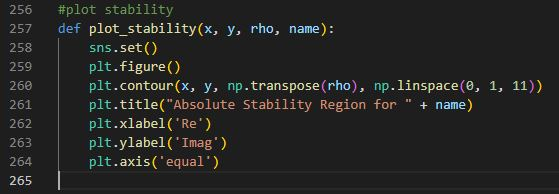
\includegraphics[width=0.75\textwidth]{FIGURES/mil4/codigo/plot2.JPG}
	\caption{Código función dibujar regiones de estabilidad.}
	\label{plot2}
\end{figure}

\subsection{stability\_regions.py}
En la siguiente figura se muestra el código de la función que calcula la región de estabilidad pasándole como argumento un método de integración numérica.
\begin{figure}[H]
	\centering
	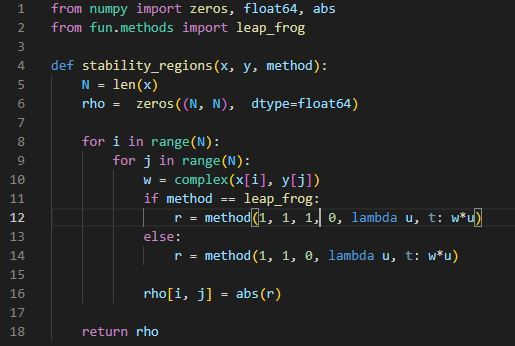
\includegraphics[width=0.75\textwidth]{FIGURES/mil4/codigo/st1.JPG}
	\caption{Código función cálculo regiones de estabilidad.}
	\label{st1}
\end{figure}


\section{Resultados de los métodos}

\subsection{Oscilador armónico lineal}
Se han realizado 3 simulaciones distintas para cada método con 3 distintos $\Delta t$. El análisis de los resultados se muestra a continuación.   

\subsubsection{Método de Euler explícito}
Como se muestra en la siguiente figura para integraciones con incrementos de tiempo altos, el error acumulado se va haciendo notable a partir de los 5 segundos de simulación. Este error se manifiesta en la amplitud tanto de la posición como de la velocidad, aumentando respecto a la solución analítica.

Conforme se va disminuyendo el incremento de tiempo utilizado en la simulación el resultado del método se asemeja más a la resolución analítica y por por lo tanto es una solución más estable.
\begin{figure}[H]
	\centering
	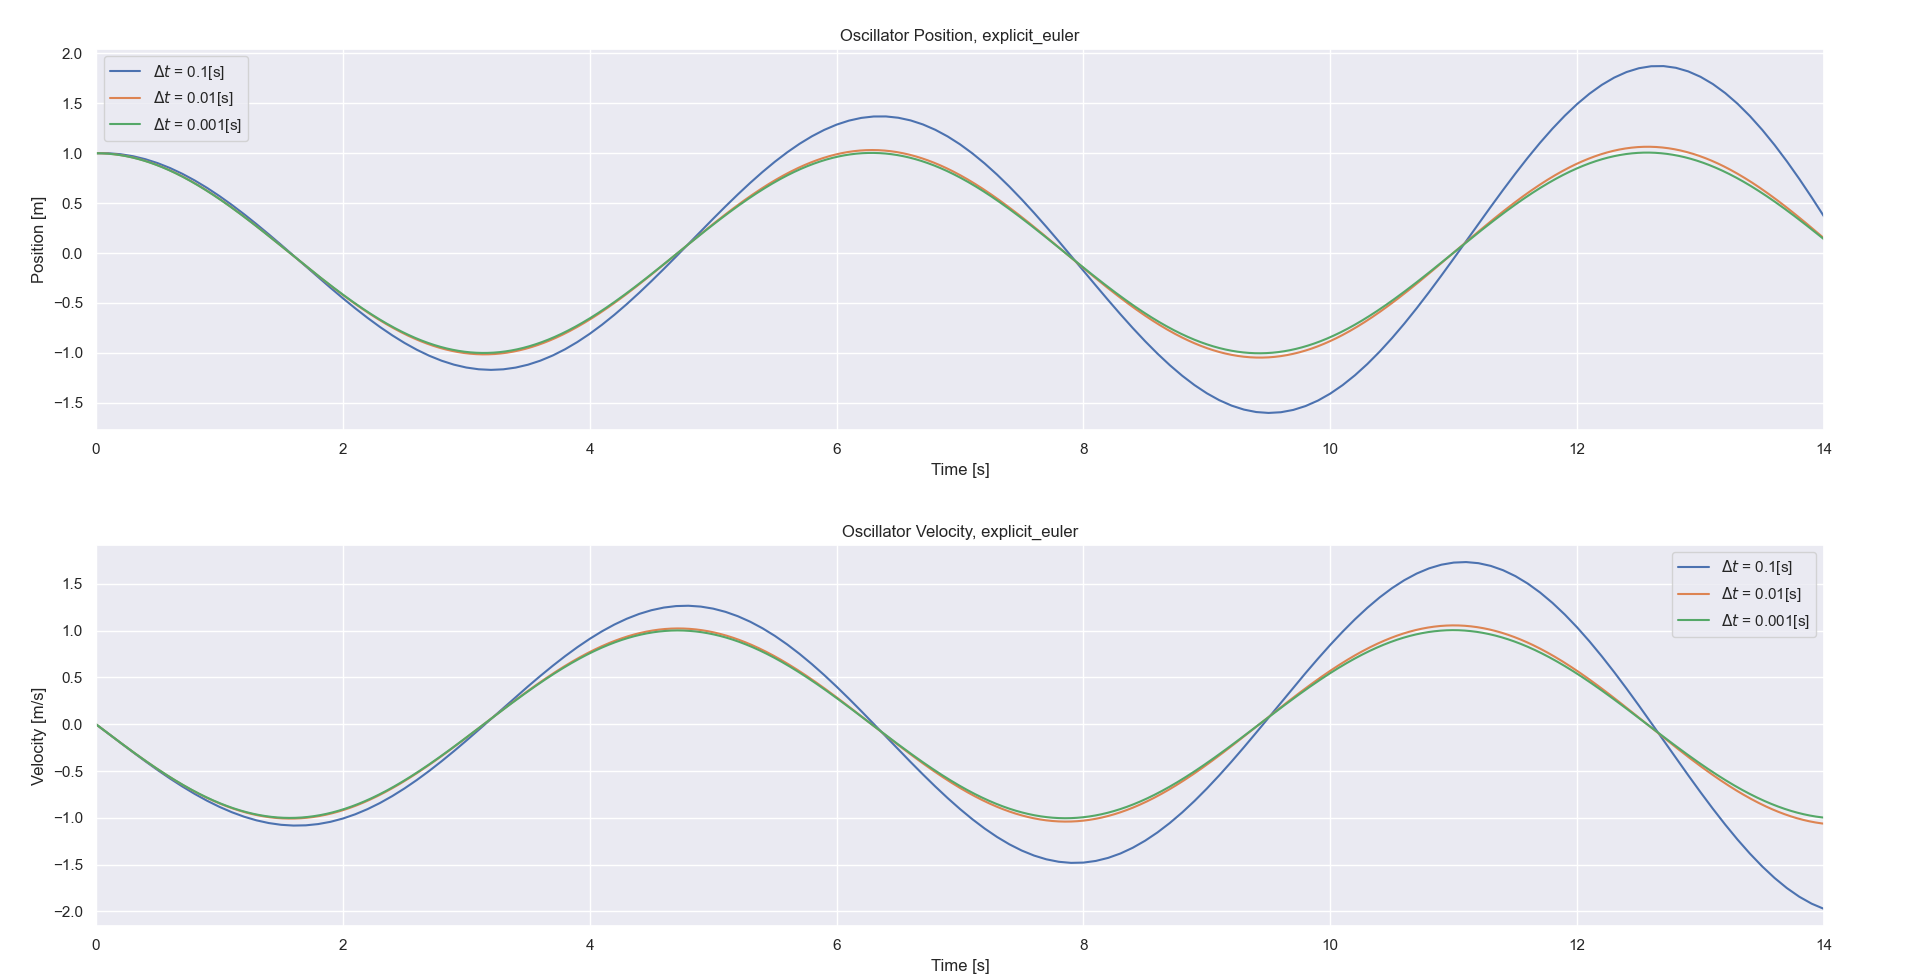
\includegraphics[width=0.95\textwidth]{FIGURES/mil4/osci_euler.png}
	\caption{Resolución oscilador con método de Euler y distintos $\Delta t$.}
	\label{osci_euler}
\end{figure}


\subsubsection{Método de Runge-Kutta de orden 4}
Este método de integración consigue obtener muy buenos resultados incluso para $\Delta t$ altos. 
\begin{figure}[H]
	\centering
	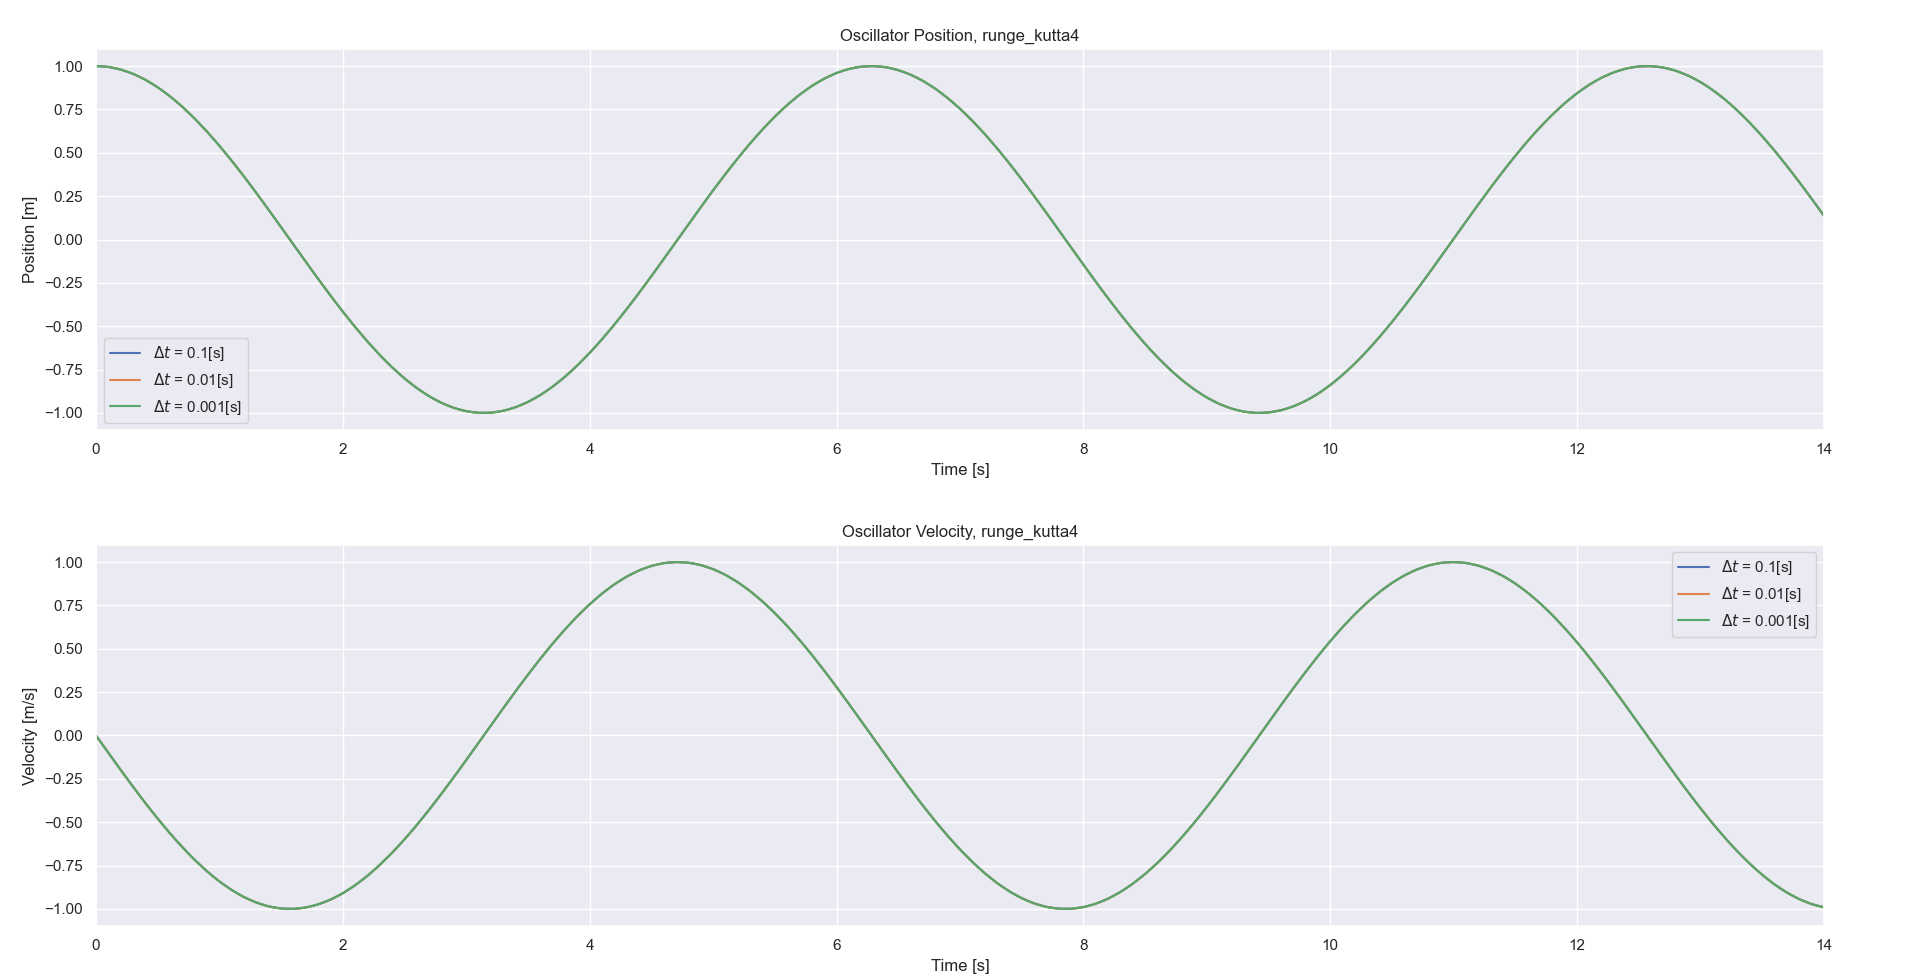
\includegraphics[width=0.95\textwidth]{FIGURES/mil4/osci_rungekutta4.png}
	\caption{Resolución oscilador con método de Runge-Kutta de orden 4 y distintos $\Delta t$.}
	\label{osci_rungekutta4}
\end{figure}


\subsubsection{Método de Euler inverso}
Como se muestra en la siguiente figura para integraciones con $\Delta t$ altos, el error acumulado se va haciendo notable a partir de los 5 segundos de simulación. Este error se manifiesta en la amplitud tanto de la posición como de la velocidad, disminuyendo respecto a la solución analítica.

Conforme se va disminuyendo el $\Delta t$ utilizado en la simulación, el resultado del método se asemeja más a la resolución analítica y por por lo tanto es una solución más estable.
\begin{figure}[H]
	\centering
	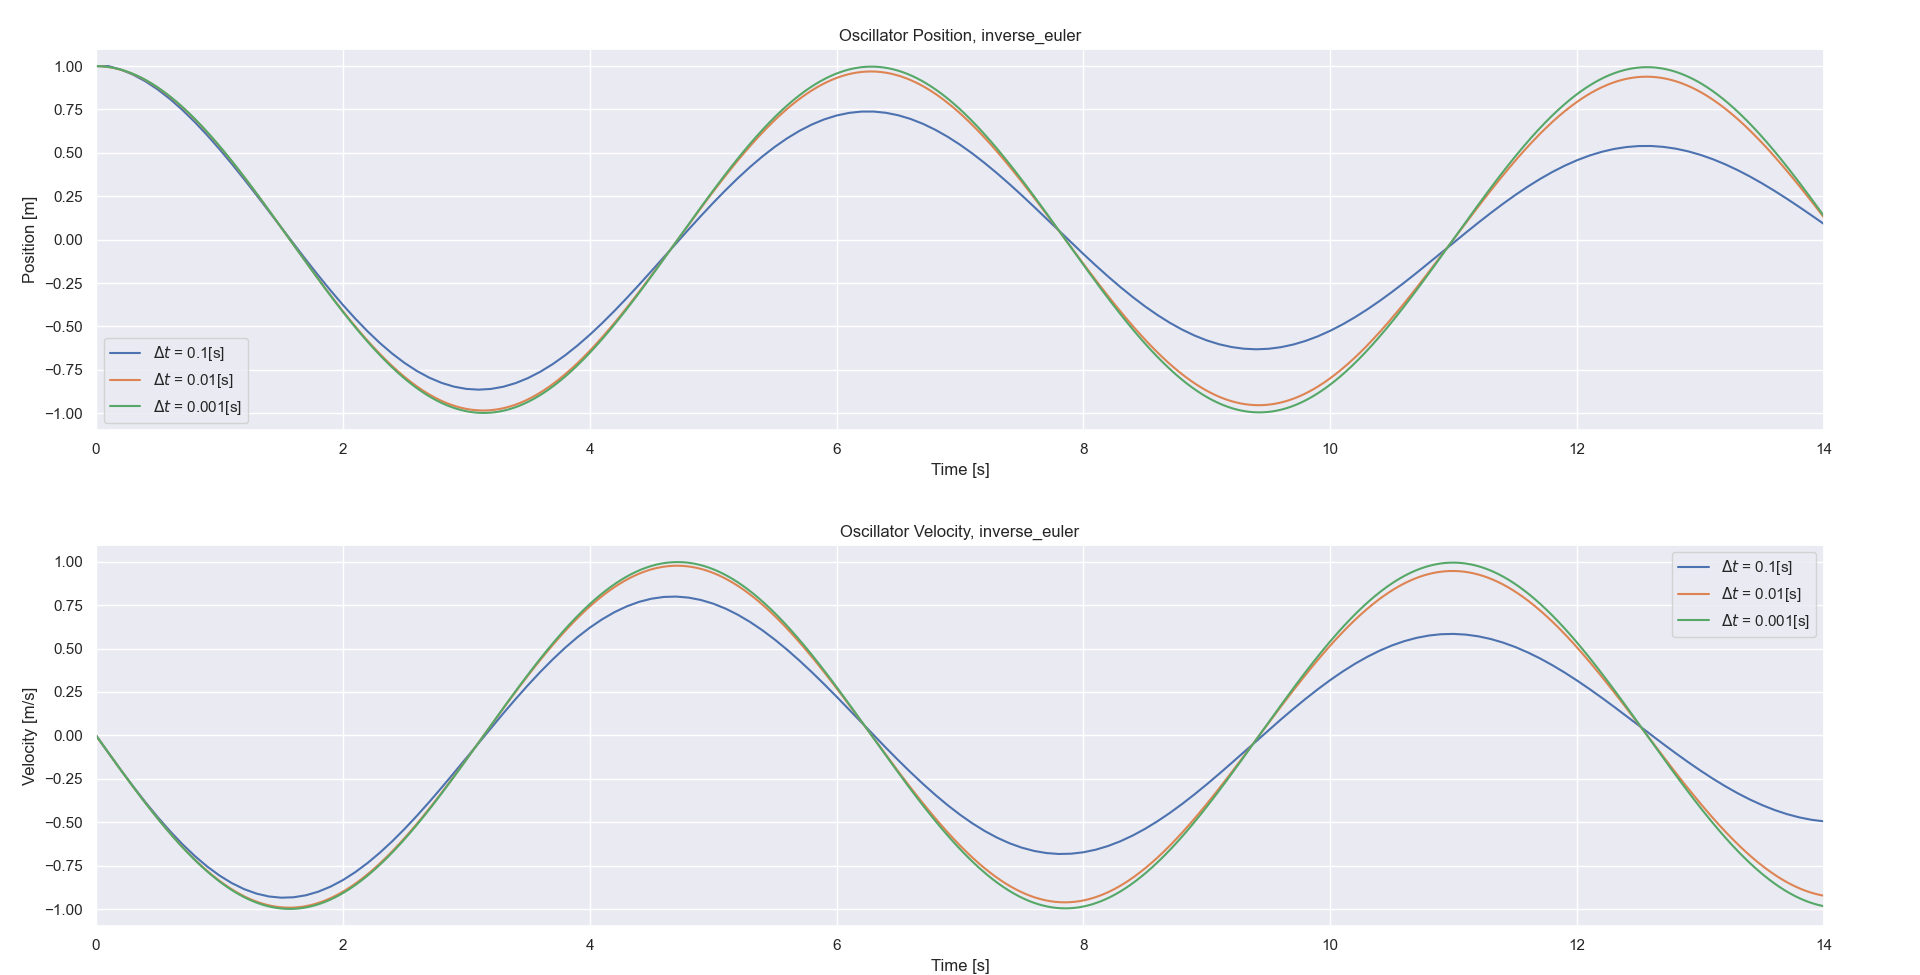
\includegraphics[width=0.95\textwidth]{FIGURES/mil4/osci_inveuler.png}
	\caption{Resolución oscilador con método de Euler inverso y distintos $\Delta t$.}
	\label{osci_inveuler}
\end{figure}


\subsubsection{Método de Crank-Nicholson}
Con este método de resolución numérico se obtienen buenos resultados incluso para incrementos de tiempo altos. Esto se traduce en que este método es bastante estable en la resolución de problemas numéricos.
\begin{figure}[H]
	\centering
	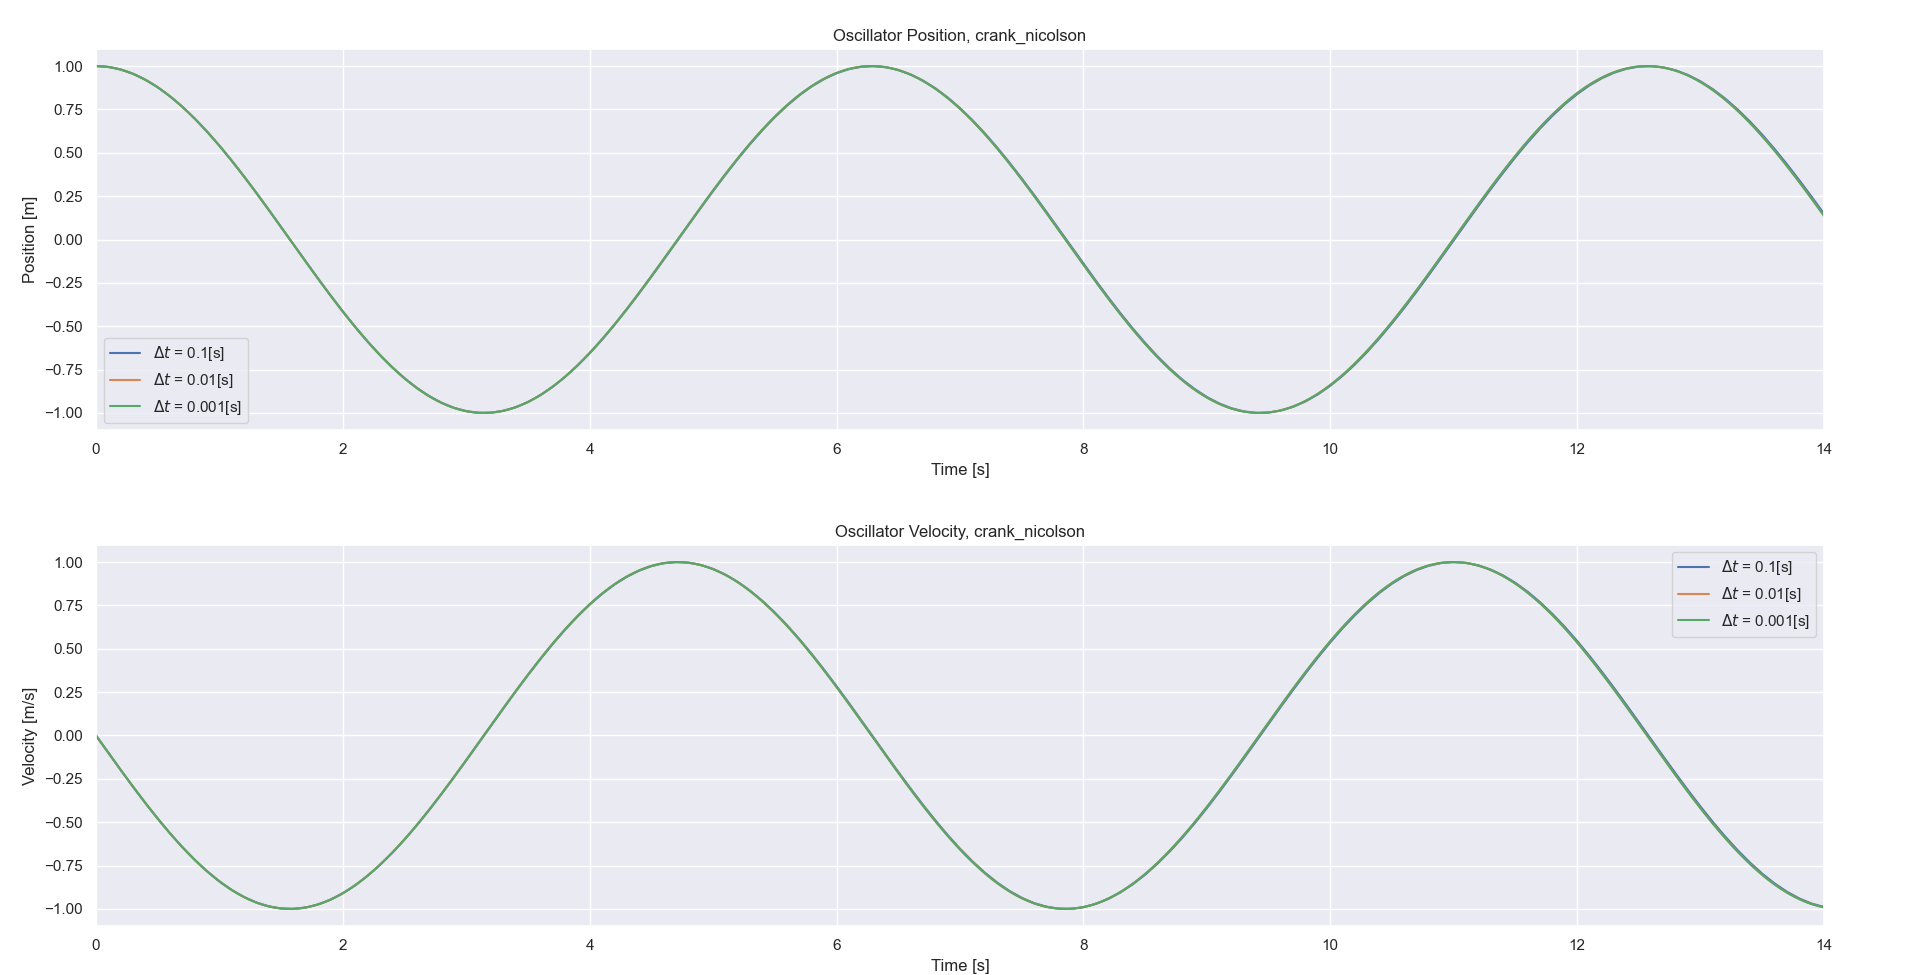
\includegraphics[width=0.95\textwidth]{FIGURES/mil4/osci_crank.png}
	\caption{Resolución oscilador con método de Crank-Nicholson y distintos $\Delta t$.}
	\label{osci_crank}
\end{figure}


\subsubsection{Método de Leap-Frog}
Con el nuevo método implementado de resolución numérica se obtienen resultados bastante buenos a partir de $\Delta t \leq 0.01 [s]$. Para incrementos de tiempo mayores se puede apreciar unos escalones entre cada paso temporal, conforme disminuimos dicho incremento de tiempo, esas "discontinuidades" desaparecen o se hacen mucho más pequeñas e imperceptibles.
\begin{figure}[H]
	\centering
	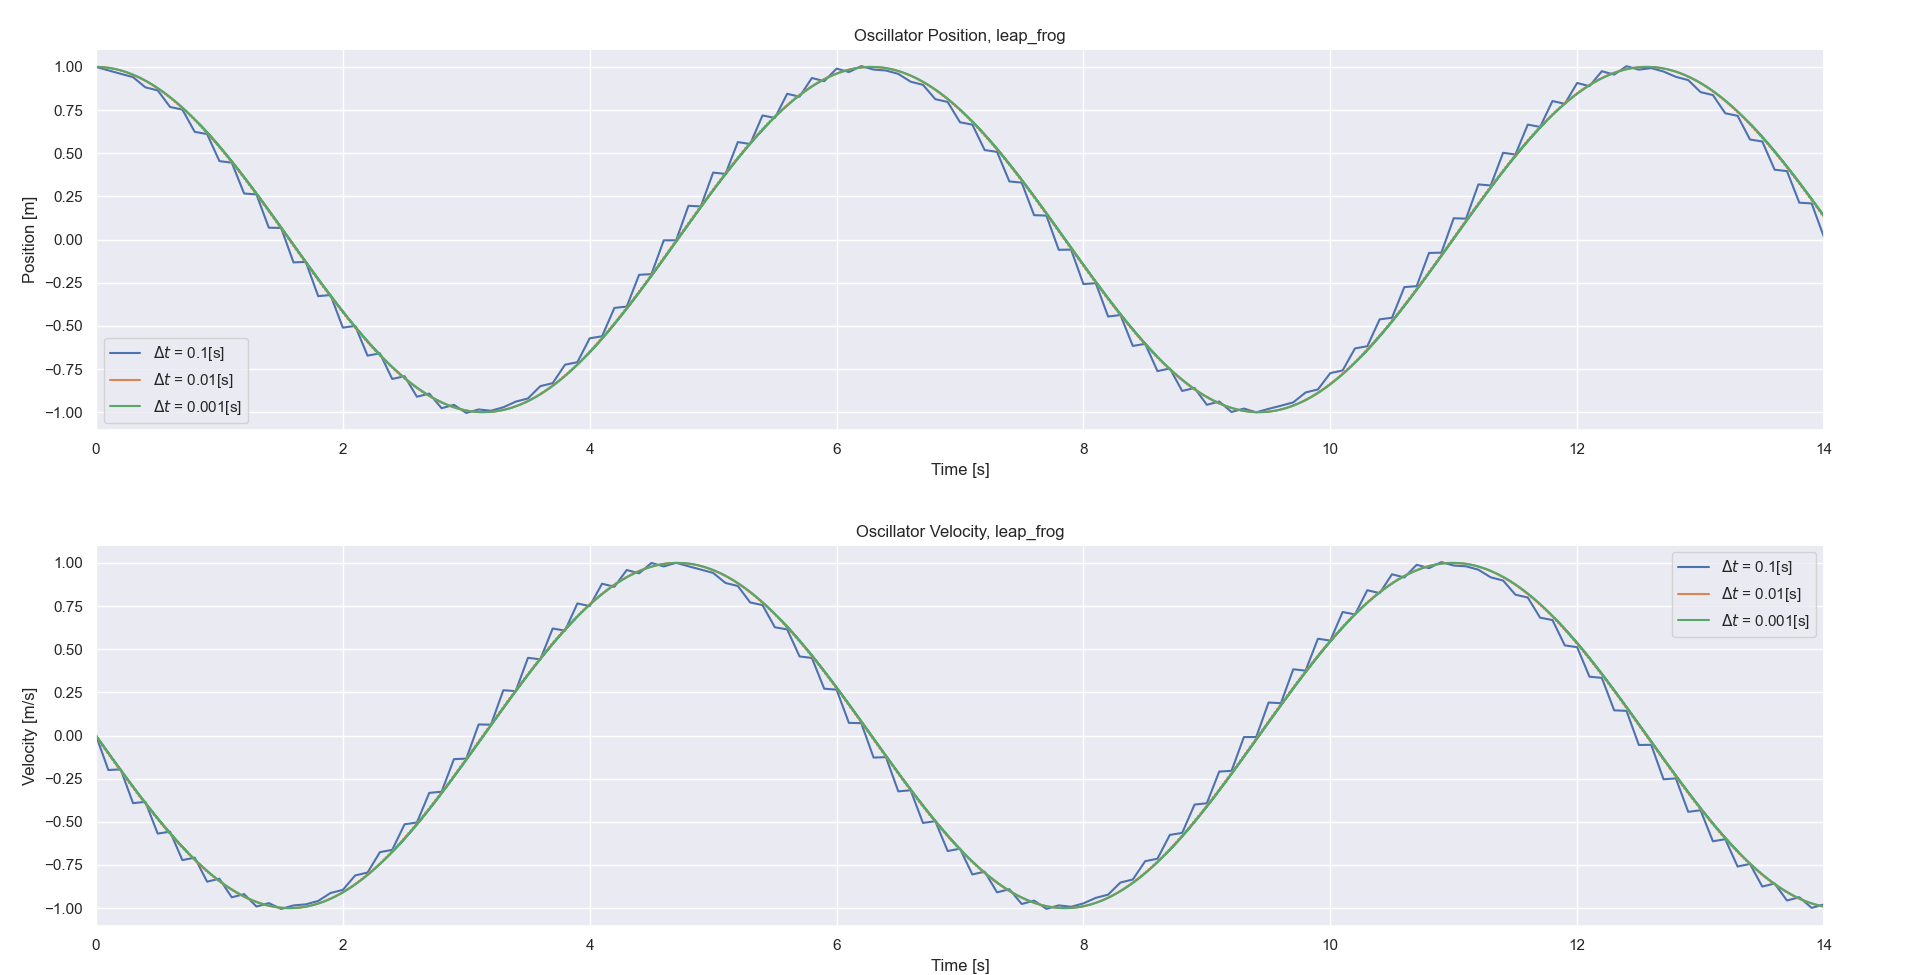
\includegraphics[width=0.95\textwidth]{FIGURES/mil4/osci_leap.png}
	\caption{Resolución oscilador con método de Leap-Frog y distintos $\Delta t$.}
	\label{osci_leap}
\end{figure}


\subsection{Regiones de estabilidad}
\subsubsection{Método de Euler explícito}
La región de estabilidad de este método es el interior de una circunferencia cuyo centro es el punto (-1, 0) en el plano complejo.

Como se muestra en la figura siguiente, en estas regiones, en el plano complejo, revelan los valores que puede asumir z (nº complejo) tal que el error en el método se comporte asintóticamente igual al error local de truncado para todo tiempo de la simulación.
\begin{figure}[H]
	\centering
	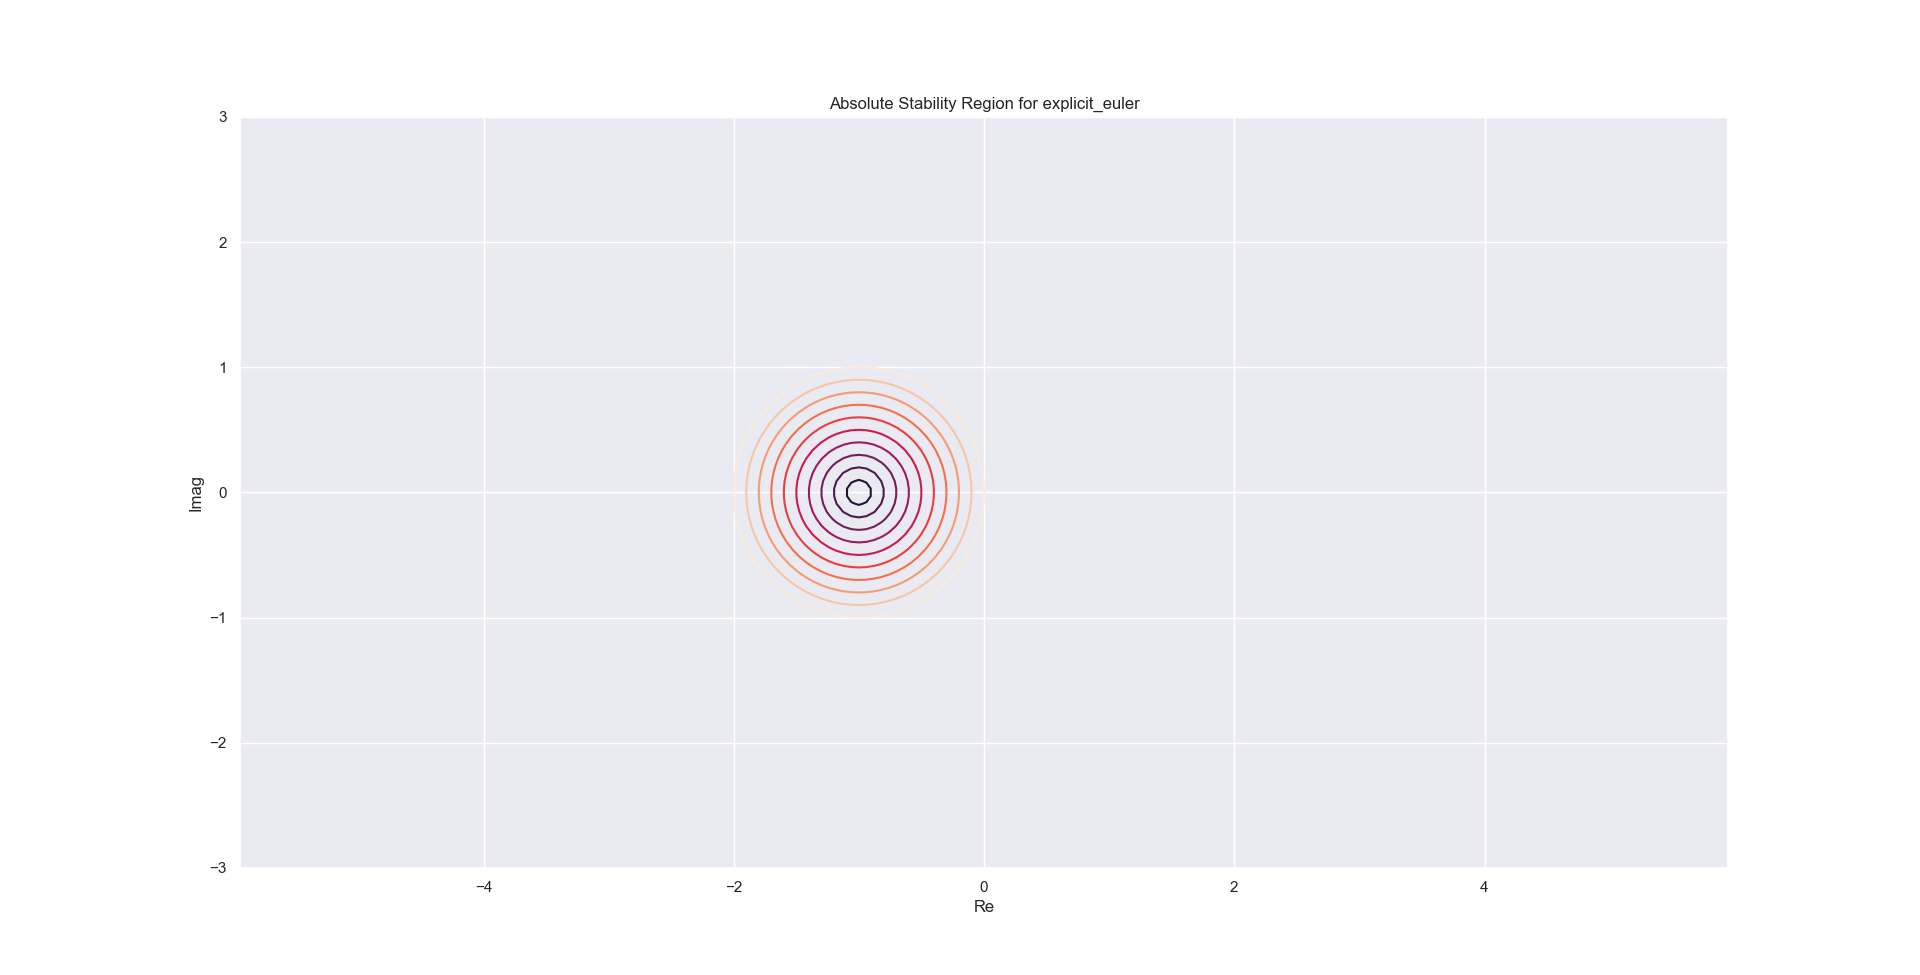
\includegraphics[width=0.8\textwidth]{FIGURES/mil4/st_euler.png}
	\caption{Región de estabilidad método de Euler.}
	\label{st_euler}
\end{figure}


\subsubsection{Método de Runge-Kutta de orden 4}
En la siguiente figura se muestra la región de estabilidad del método de Runge-Kutta, como puede observarse se trata de una región bastante amplia que hace que este método genere soluciones bastante estables incluso con incrementos de tiempo altos.
\begin{figure}[H]
	\centering
	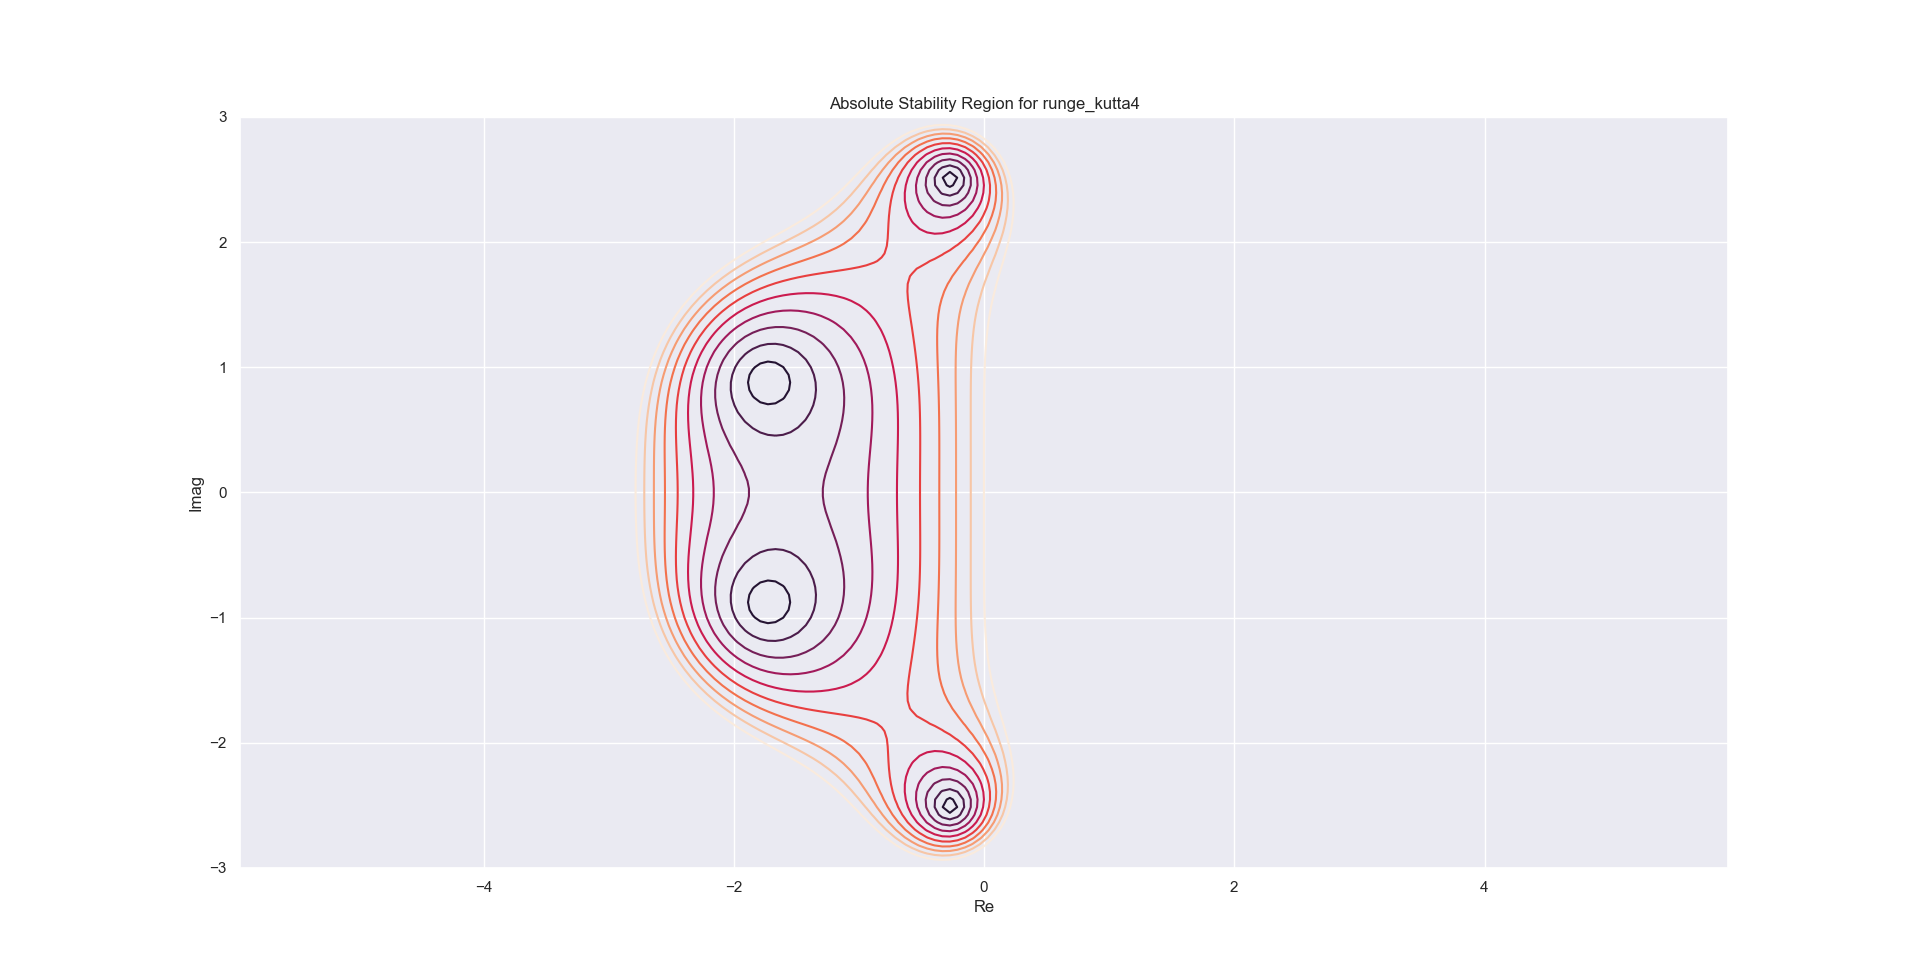
\includegraphics[width=0.8\textwidth]{FIGURES/mil4/st_rungekutta4.png}
	\caption{Región de estabilidad método de Runge-Kutta de orden 4.}
	\label{st_rungekutta4}
\end{figure}


\subsubsection{Método de Euler inverso}
En este caso la región de estabilidad es el caso contrario que para el método de Euler explícito. Esta se sitúa en el exterior de una esfera centrada en el punto (1, 0) del plano complejo. 
\begin{figure}[H]
	\centering
	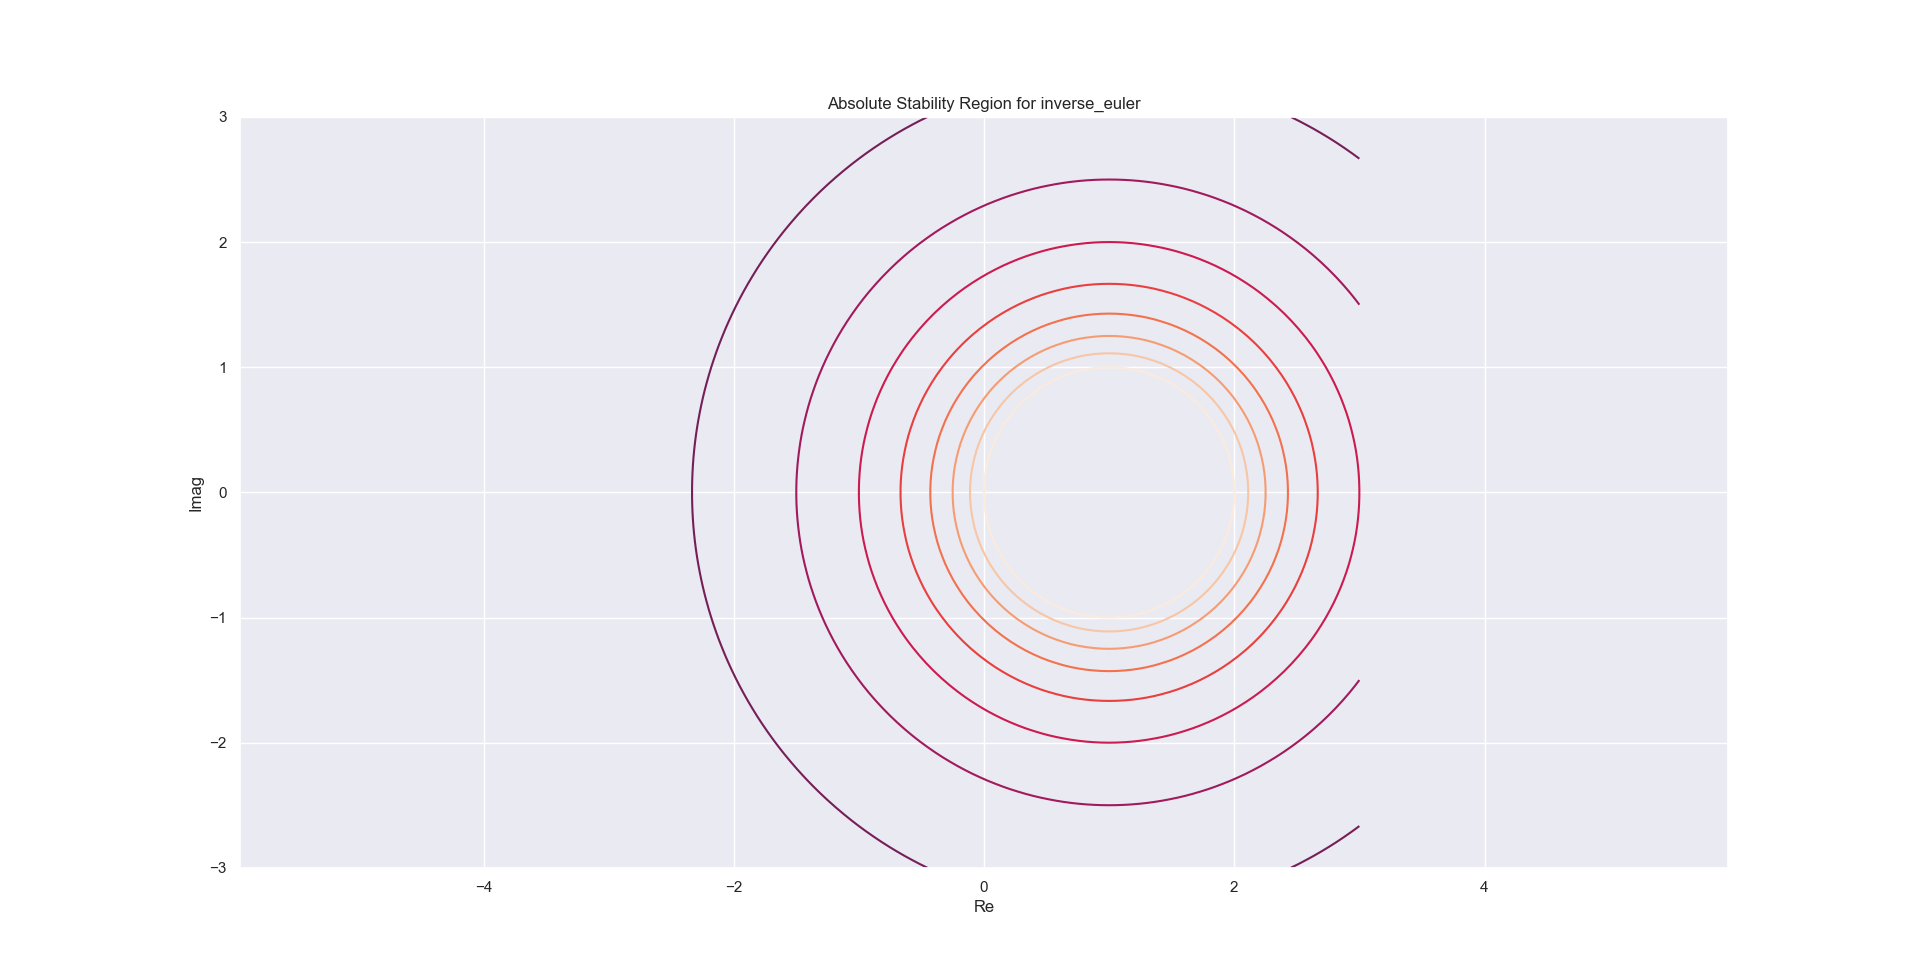
\includegraphics[width=0.8\textwidth]{FIGURES/mil4/st_inveuler.png}
	\caption{Región de estabilidad método de Euler inverso.}
	\label{st_inveuler}
\end{figure}


\subsubsection{Método de Crank-Nicholson}
En la siguiente figura se muestra la región de estabilidad del método de Crank-Nicholson, la cual está perfectamente acotada en la parte negativa del eje Real del plano complejo. Esto hace que este método genere soluciones bastante estables incluso para incrementos de tiempo altos.
\begin{figure}[H]
	\centering
	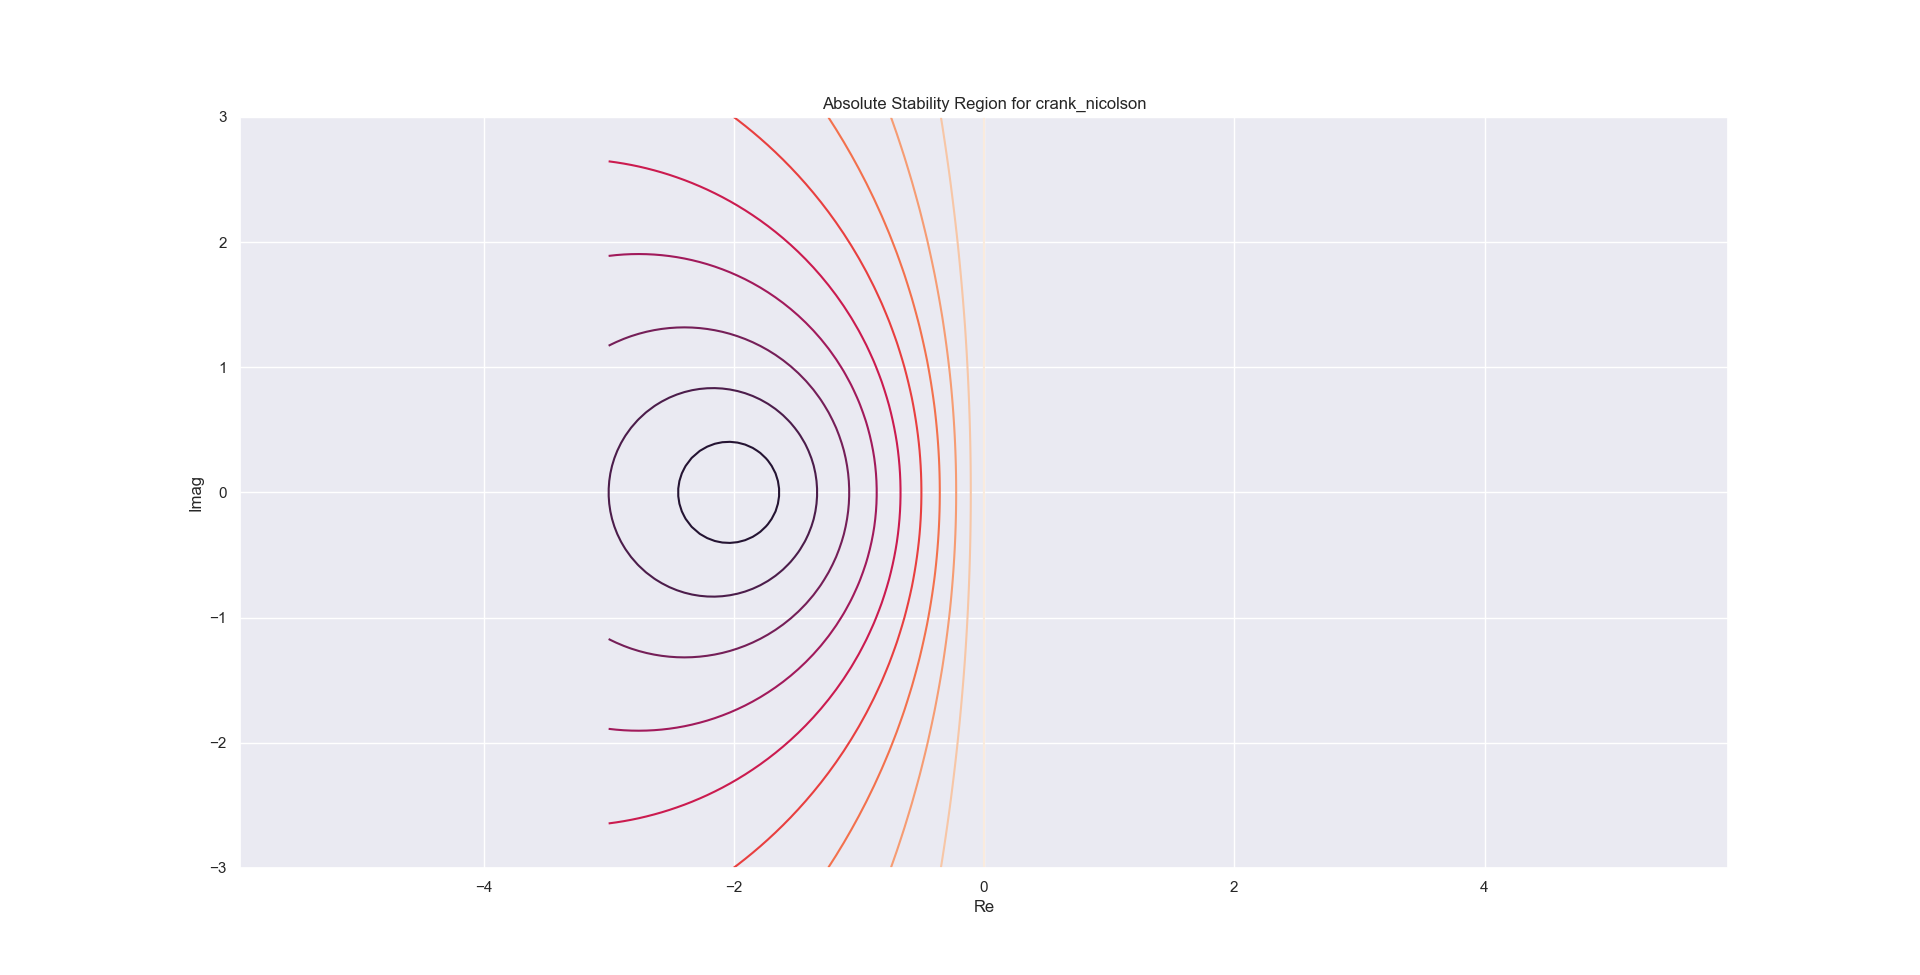
\includegraphics[width=0.8\textwidth]{FIGURES/mil4/st_crank.png}
	\caption{Región de estabilidad método de Crank-Nicholson.}
	\label{st_crank}
\end{figure}


\subsubsection{Método de Leap-Frog}
En la siguiente figura se muestra la región de estabilidad absoluta del método de Leap-Frog.
\begin{figure}[H]
	\centering
	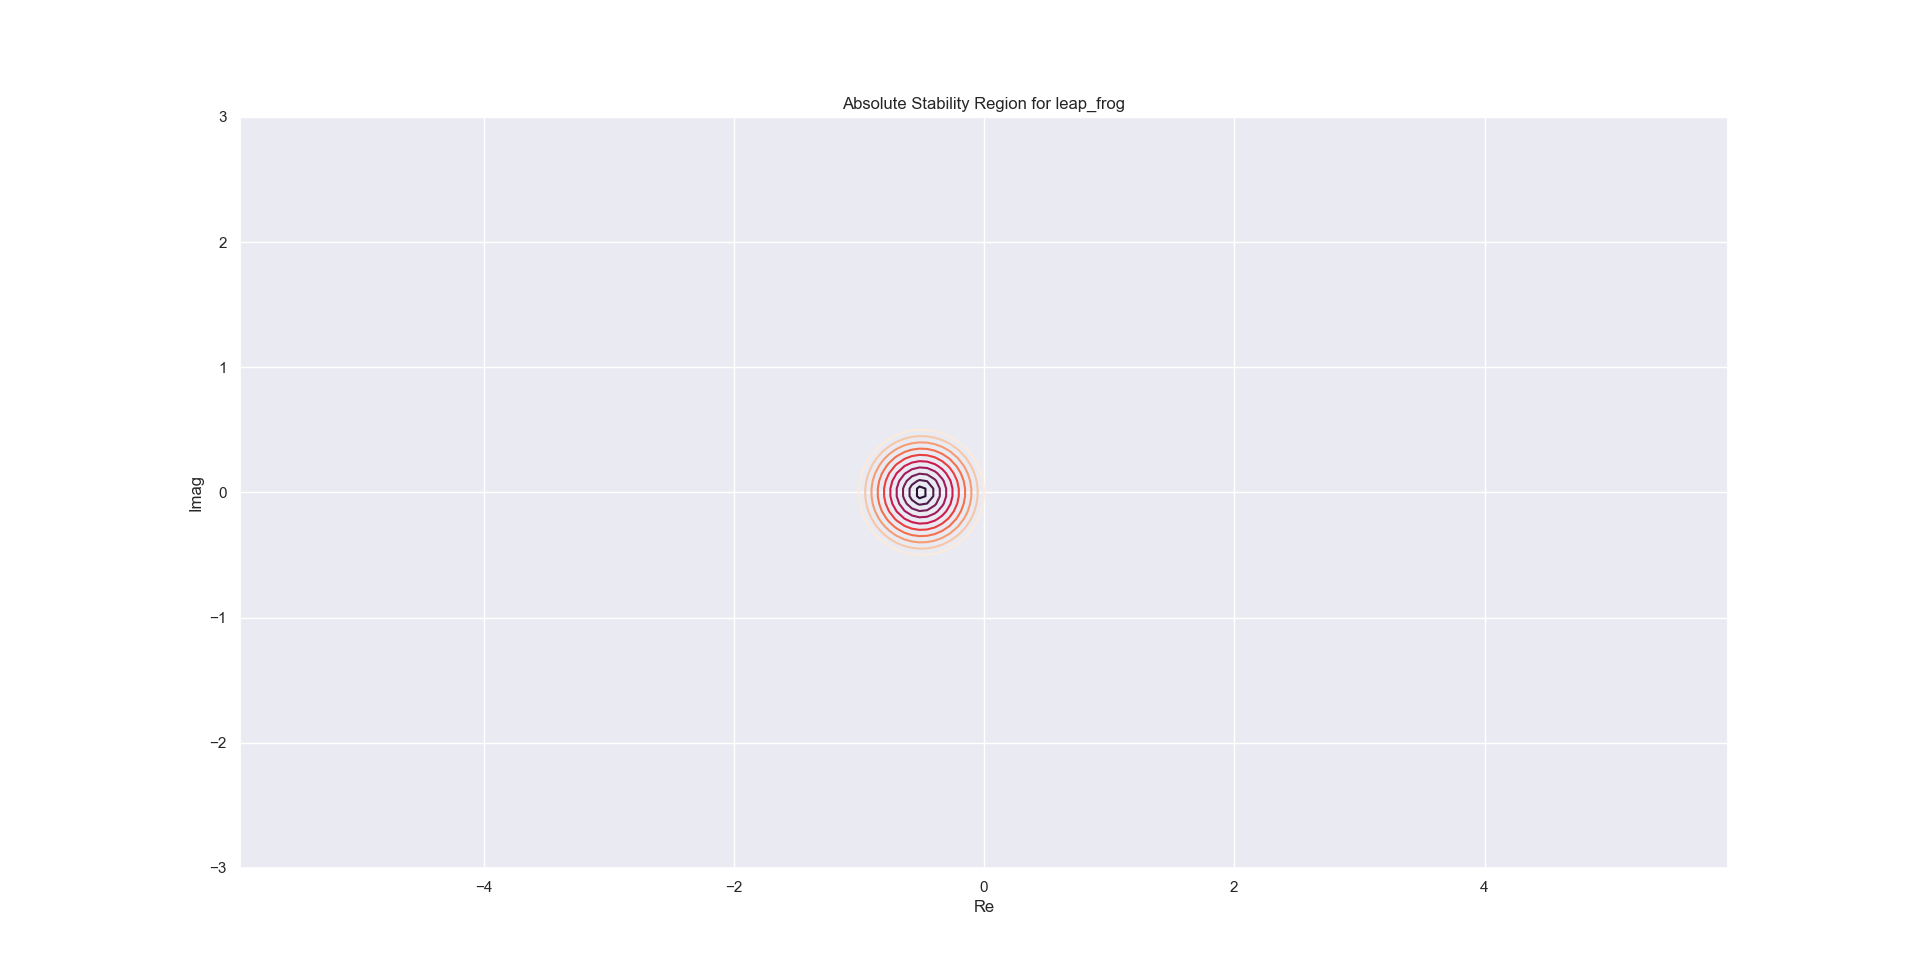
\includegraphics[width=0.8\textwidth]{FIGURES/mil4/st_leap.png}
	\caption{Región de estabilidad método de Leap-Frog.}
	\label{st_leap}
\end{figure}



\section{Conclusiones}
%Suuuuuu
Se ha utilizado un programa externo denominado $software\_design$ para la obtención del diagrama de bloques de este hito y se utilizará para los siguientes también. Este software es muy útil puesto que permite generar un mapa general de todos los módulos implicados en el programa y conocer de antemano las relaciones entre ellos.



\end{document}
